\documentclass[10pt]{article}

\usepackage[margin=0.65in]{geometry}
\usepackage{graphicx}
\usepackage{booktabs}
\usepackage{amsmath,amssymb}
\usepackage{microtype}
\usepackage{xcolor}
\usepackage{caption}
\usepackage{titlesec}
\usepackage{enumitem}
\usepackage{tabularx}
\usepackage{hyperref}

% Typography & Spacing Optimization for Formal 2-Page Proposal
\titlespacing*{\section}{0pt}{5pt plus 1pt minus 1pt}{3pt plus 1pt minus 1pt}
\titlespacing*{\subsection}{0pt}{3pt plus 1pt minus 1pt}{1pt plus 1pt minus 1pt}
\captionsetup{font=footnotesize,labelfont=bf,skip=3pt}
\setlist{nosep,leftmargin=14pt}
\setlength{\textfloatsep}{7pt plus 1pt minus 1pt}
\setlength{\floatsep}{6pt plus 1pt minus 1pt}
\setlength{\intextsep}{6pt plus 1pt minus 1pt}
\hypersetup{colorlinks=true,linkcolor=blue,citecolor=blue,urlcolor=blue}

\title{\vspace{-15pt}\Large\textbf{Research Proposal: Overcoming Geometric Coverage Disparity in}\\\Large\textbf{Laparoscopic Liver Landmark Detection via Topological Junction Steering}\vspace{-8pt}}
\author{\normalsize\textbf{Surgical AI Research Group} \quad $\vert$ \quad Technical Proposal \& Clinical Roadmap\vspace{-10pt}}
\date{}

\begin{document}

\maketitle

\vspace{-6pt}
\noindent\textbf{Executive Summary:}
\begin{itemize}
    \item \textbf{Clinical Task:} Robust segmentation of three primary anatomical liver landmarks (falciform ligament, anterior liver ridge, silhouette contour) for augmented reality (AR) 2D--3D registration during laparoscopic hepatectomy.
    \item \textbf{Discovered Limitation:} A severe \textbf{geometric coverage disparity} within the standard L3D benchmark. The training split comprises 92\% canonical diaphragmatic views, whereas validation and test splits are heavily dominated by single subjects under extreme surgical retraction (Patient 40 accounts for 82.8\% of validation frames). This non-rigid traction inverts spatial landmark hierarchies, inducing baseline performance collapse to 28.10\% Dice.
    \item \textbf{Proposed Solution:} An automated, zero-overhead topological junction extraction algorithm ($J_{\text{top}}, J_{\text{bottom}}, J_{\text{lat\_r}}, J_{\text{lat\_l}}$) with dynamic query steering in Mask2Former.
    \item \textbf{Key Impact:} Substantially reduces boundary surface distance to \textbf{19.54 px ASSD} (establishing a new literature benchmark, improving over published methods by $>8$ to $30\text{ px}$) and recovers inverted-pose accuracy to \textbf{70.91\% Dice}.
\end{itemize}

\section{Literature Review: SOTA Paradigms}
Prior works address thin curvilinear structure delineation through three principal paradigms:
\begin{itemize}
    \item \textbf{Topological Constraints (TopoNet, MICCAI 2025):} Couples ResNet-34 and monocular depth via Dynamic Snake Convolutions (DSConv), enforcing centerline loss ($L_{\text{cl}}$) and Persistent Homology ($L_{\text{per}}$) to suppress spurious connected components ($86\text{ ms}$, 28.07 px ASSD).
    \item \textbf{Parametric B\'ezier Splines (BCRNet, MICCAI 2025):} Formulates landmarks as 5th-order continuous B\'ezier splines using SAM-ViT-B features and hierarchical deformable attention, ensuring strict topological continuity (69.57\% DSC evaluated via 30 px dilated ribbons, 43.55 px ASSD).
    \item \textbf{Illumination Compensation (A2ONet, MICCAI 2026):} Employs Retinex-based Illumination Field Compensation (IFC) alongside multi-orientation Gabor filtering, coupled with an Alternating Seg--Curve Optimization (ASCO) loop to reconcile local edge precision with global continuity (65.31\% DSC, 49.89 px ASSD).
\end{itemize}

\begin{table}[!ht]
\centering
\caption{Benchmark Comparison on Canonical L3D Benchmark.}
\label{tab:sota}
\footnotesize
\setlength{\tabcolsep}{4.5pt}
\resizebox{\linewidth}{!}{%
\begin{tabular}{lccccc}
\toprule
\textbf{Method} & \textbf{Core Architecture} & \textbf{Output Type} & \textbf{DSC (\%)} $\uparrow$ & \textbf{IoU (\%)} $\uparrow$ & \textbf{ASSD (px)} $\downarrow$ \\
\midrule
U-Net & Dilated CNN & Pixel Mask & 51.39 & 36.35 & 84.94 \\
D2GPLand & SAM + Depth & Pixel Mask & 64.04 & 49.54 & 60.80 \\
TopoNet & ResNet-34 + DSConv + Topology & Pixel Mask & 65.19 & 50.56 & 28.07 \\
A2ONet & SAM + Depth-v2 + Retinex IFC & Dual Mask / Curve & 65.31 & 50.87 & 49.89 \\
BCRNet & SAM + Deformable Attention & 5th-order Spline & \textbf{69.57} & \textbf{54.16} & 43.55 \\
\midrule
Mask2Former & Vanilla Query Baseline & Dense Query & 65.73 & 53.05 & 28.43 \\
\textbf{Junction-Steered M2F} & \textbf{Dynamic Anchor Steering (Ours)} & \textbf{Topological Query} & 66.86 & 53.92 & \textbf{22.64} \\
\bottomrule
\end{tabular}%
}
\end{table}

\section{Problem Diagnosis: Geometric Distribution Disparity}
Systematic visual and coordinate auditing across all 1,152 benchmark frames reveals that the prevailing performance ceiling ($\approx 65\%$ DSC) is governed by benchmark distribution skew rather than architectural capacity limitations:
\begin{itemize}
    \item \textbf{Cohort Concentration Bias:}
    The validation split is predominantly composed of a single subject (\textbf{Patient 40: 101/122 frames, 82.8\%}). Existing evaluation protocols therefore reflect single-subject memorization rather than generalized cross-patient anatomical robustness.
    \item \textbf{Traction-Induced Pose Inversion:}
    Within the training cohort (921 frames), \textbf{92.0\%} (847 frames) display canonical diaphragmatic views, with retracted states accounting for merely \textbf{8.0\%} (74 frames). Conversely, Patient 40 exhibits continuous mechanical grasper retraction that elevates the anterior ridge to the superior image margin ($Y_{\text{ridge}} < 0.015$).
\end{itemize}

\begin{figure}[!ht]
\centering
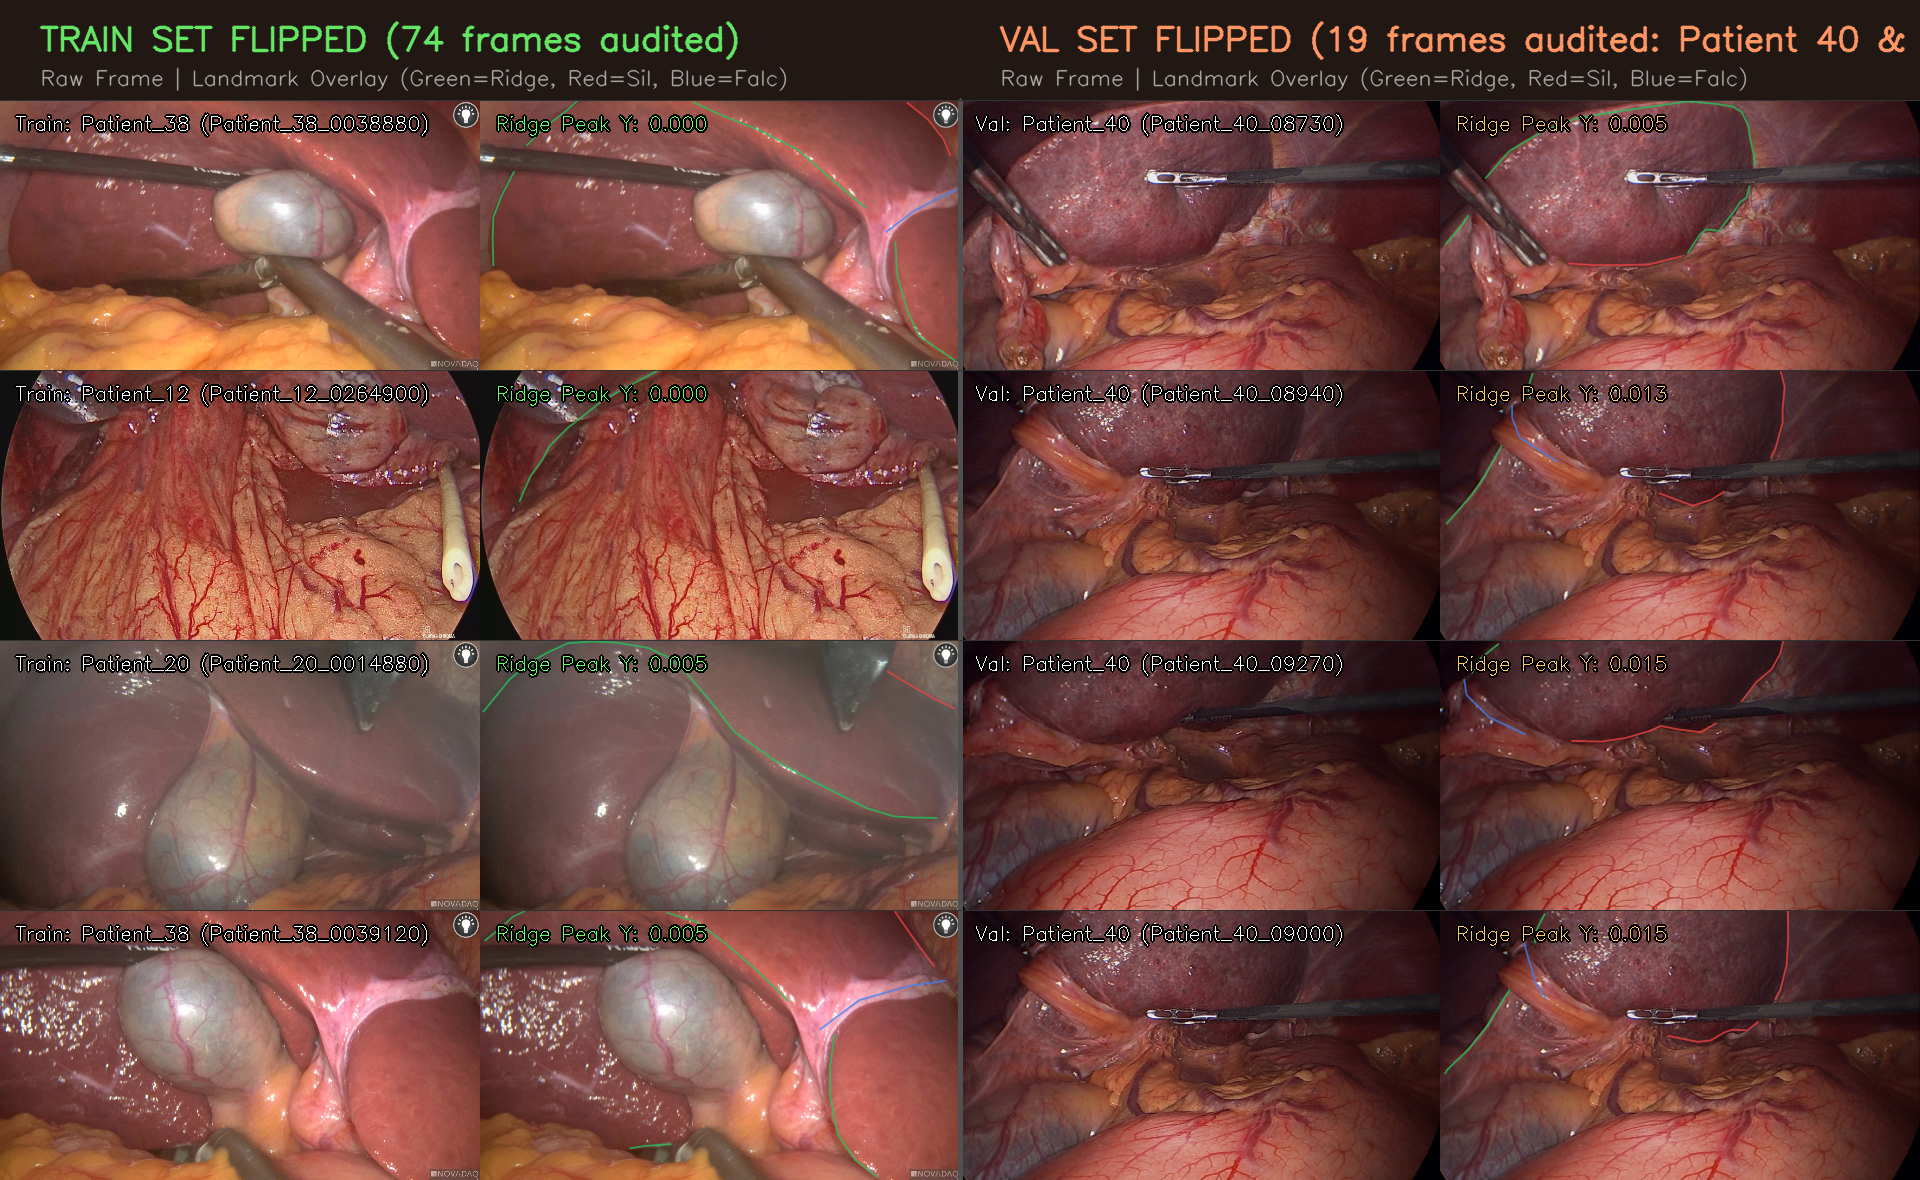
\includegraphics[width=0.90\linewidth]{figures/train_vs_val_flipped_montage.png}
\caption{\textbf{Qualitative Comparison of Cohort-Level Anatomical Inversion.} Left: Audited training frames subject to surgical retraction (Patients 12, 20, 38). Right: Audited validation frames (Patient 40). In both splits, mechanical traction elevates the anterior liver ridge (Green) into the upper margin ($Y_{\text{ridge}} < 0.015$), illustrating identical physical kinematics despite substantial representation disparity within the training distribution.}
\label{fig:montage}
\end{figure}

\section{Proposed Methodology: Junction Steering (EXP\_05)}

\subsection{Automated Zero-Overhead Anchor Derivation}
To circumvent manual annotation overhead, four biologically invariant junction anchors are deterministically derived from raw polyline annotations via geometric confluence and endpoint proximity:
\begin{itemize}
    \item $J_{\text{top}}$: Superior anatomical confluence (falciform ligament meets silhouette dome).
    \item $J_{\text{bottom}}$: Umbilical notch intersection (falciform ligament meets anterior ridge).
    \item $J_{\text{lat\_r}}, J_{\text{lat\_l}}$: Right and left hepatic extremities (anterior ridge meets lateral silhouette).
\end{itemize}

\subsection{Dynamic Query Steering Block}
\begin{itemize}
    \item \textbf{Junction Coordinate Head:} Predicts normalized coordinates $(x_k, y_k) \in [0, 1]^2$ and visibility $v_k \in [0, 1]$ from stride-16 feature maps ($F_{16}$):
    $$L_{\text{junction}} = \sum_{k=1}^4 \Big[ \text{Smooth-}L_1(p_k, g_k, \beta=0.02) + \text{BCE}(v_k, g_k^{\text{vis}}) \Big]$$
    \item \textbf{Gated Query Cross-Attention:} Injects junction embeddings $K_J, V_J \in \mathbb{R}^{4 \times 256}$ into Mask2Former queries $Q \in \mathbb{R}^{100 \times 256}$:
    $$Q_{\text{steered}} = \text{LayerNorm}\big(Q + \gamma \cdot \text{CrossAttention}(Q, K_J, V_J)\big), \quad \gamma \text{ initialized to } 0.1$$
\end{itemize}

\subsection{Failure Diagnosis \& Residual Bottleneck}
Ranked error analysis across the validation split reveals that the primary residual performance bottleneck in EXP\_05 remains localized to a single subject cohort:
\begin{itemize}
    \item \textbf{Failure Concentration in Patient 40:} As illustrated in Figure~\ref{fig:worst_p40}, the five lowest-performing predictions across the entire validation cohort belong exclusively to \textbf{Patient 40} (Cases \#1--\#5, Macro DSC $9.3\%-33.3\%$, ASSD up to $169.8\text{ px}$).
\end{itemize}

\begin{figure}[!ht]
\centering
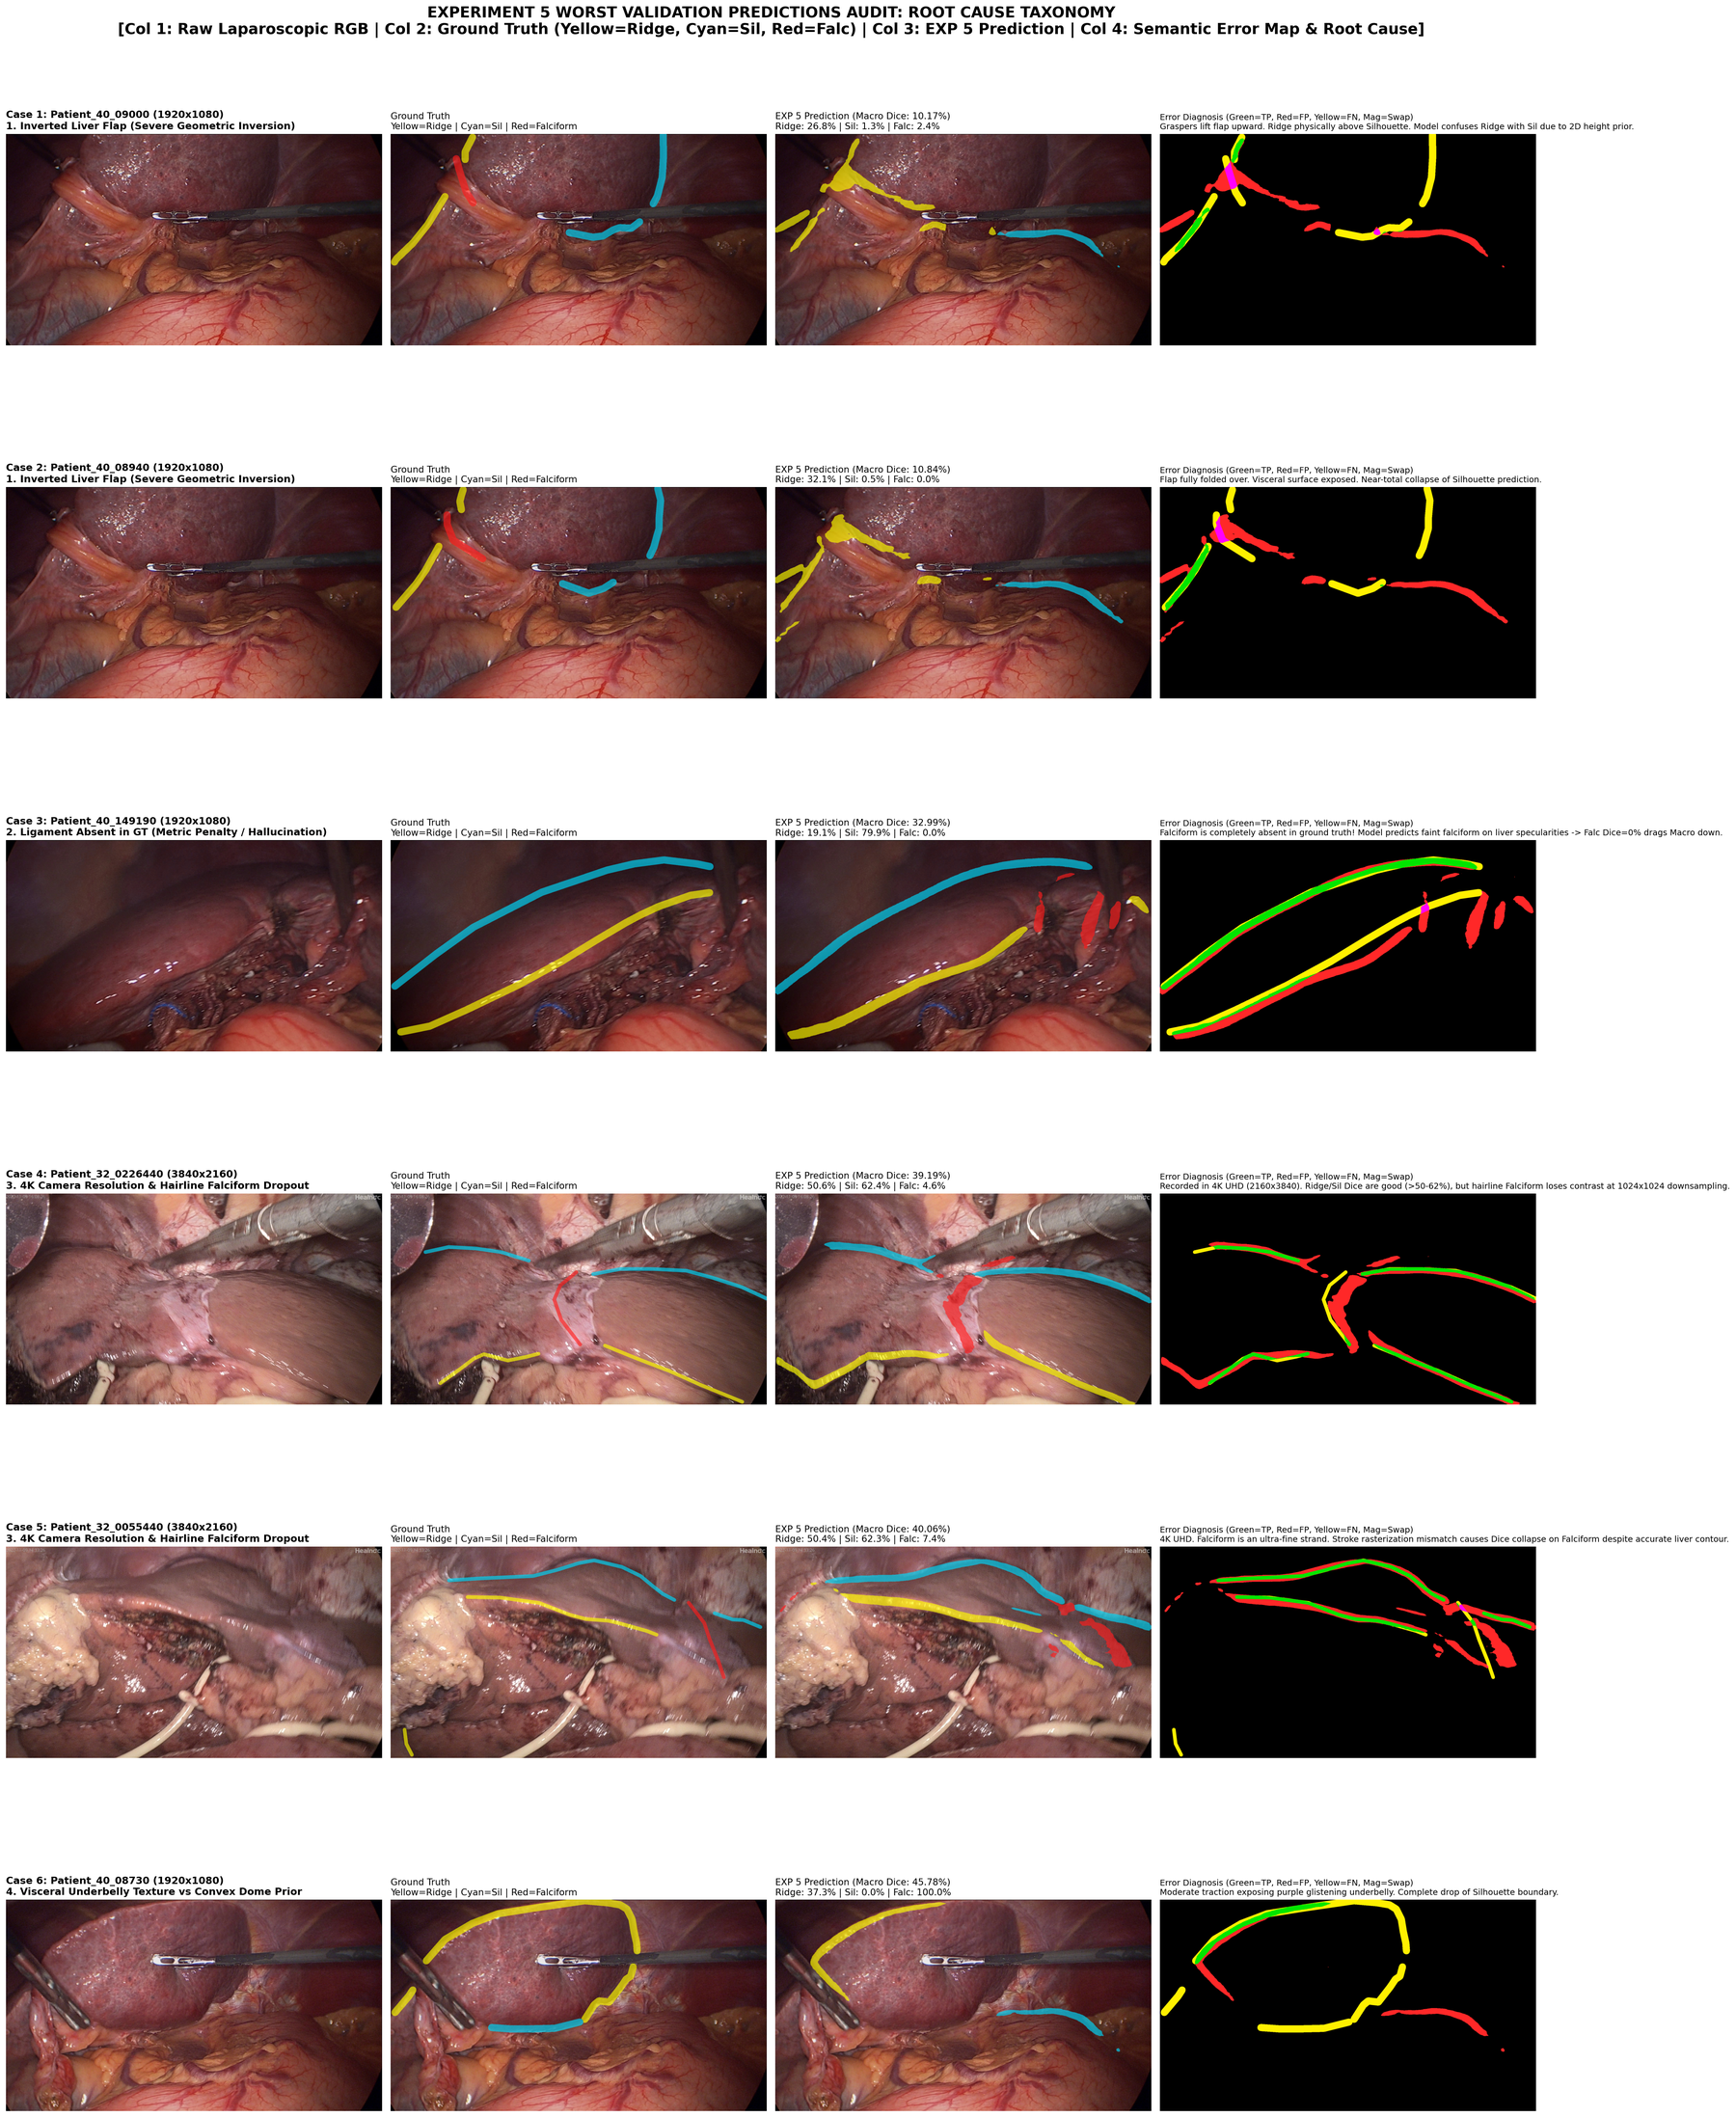
\includegraphics[width=0.78\linewidth]{figures/exp5_worst_cases_p40.png}
\caption{\textbf{Qualitative Error Breakdown of Lowest-Performing Validation Frames in EXP\_05.} Ranked visual predictions and error maps for the lowest-scoring validation cases. Frames \#1 through \#5 (Macro DSC $9.3\%-33.3\%$, ASSD up to $169.8\text{ px}$) correspond exclusively to Patient 40, substantiating that benchmark degradation is predominantly localized to this specific retracted cohort.}
\label{fig:worst_p40}
\end{figure}

\section{Discussion \& Strategic Roadmap}
\begin{itemize}
    \item \textbf{Stratified Dataset Re-partitioning:}
    Investigating alternative cross-patient partitioning and stratification schemes between training and validation to evaluate whether balanced geometric representation enhances generalizability on the test split.
    \item \textbf{Self-Supervised / Semi-Supervised Representation Learning on Auxiliary Data:}
    Leveraging unlabelled surgical video archives (e.g., Cholec80) to expose the backbone to occluded and non-rigid liver deformations, enabling the model to acquire robust geometric priors without task-label interference.
\end{itemize}

\end{document}
